\documentclass{article}
\usepackage{svg}
\usepackage{caption}
\usepackage{subcaption}
\usepackage{graphicx}
\usepackage{tabularx}

\usepackage[margin=1in]{geometry} % for 1 inch side panels


\begin{document}

\begin{titlepage}
    \centering
    \vspace*{0cm}
    {\scshape\Large Frankfurt University of Applied Sciences}\\[3cm]
    {\huge\bfseries ABCD}\\[8cm]
    {\Large\itshape Group 6:}\\
    {\Large\itshape Hermon Giikael, Howard-Yi Hong Soon, Jiwon Won, Lars Friese, Marc Roemer, Stefan Nguyen}\\[4cm]
    Supervisor:\\
    Jörg Schäfer\\[3cm]
    {\large \today}
\end{titlepage}

\tableofcontents
\newpage

\section{Hermon Gimikael}

	\subsection{Requirement1}
		\begin{figure}[h!]
		    \centering
		    \captionsetup{labelformat=empty}
		    \caption{Your caption}
		    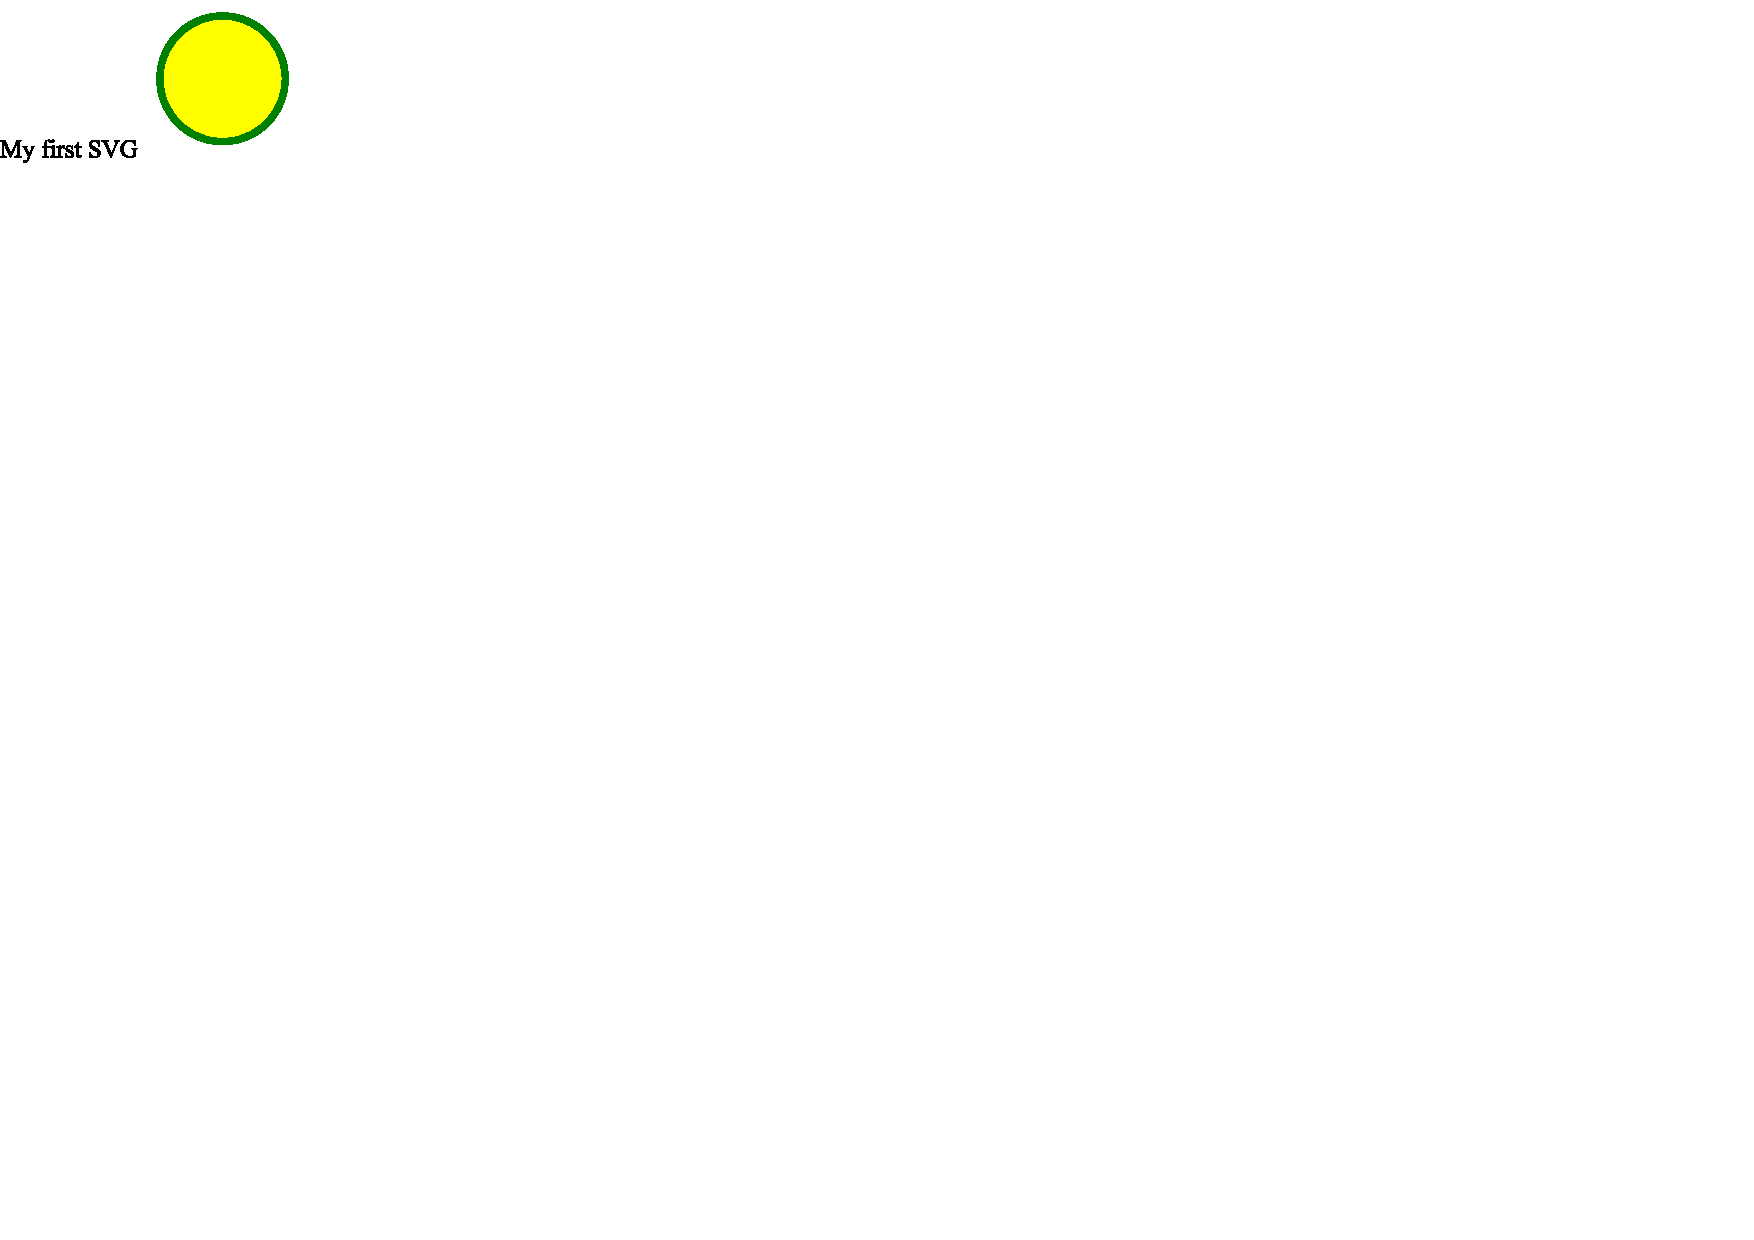
\includegraphics[width=\textwidth, angle=0]{Kreis2.pdf}
		\end{figure}
		\newpage
		\begin{figure}[h!]
		    \centering
		    \captionsetup{labelformat=empty}
		    \caption{Your caption}
		    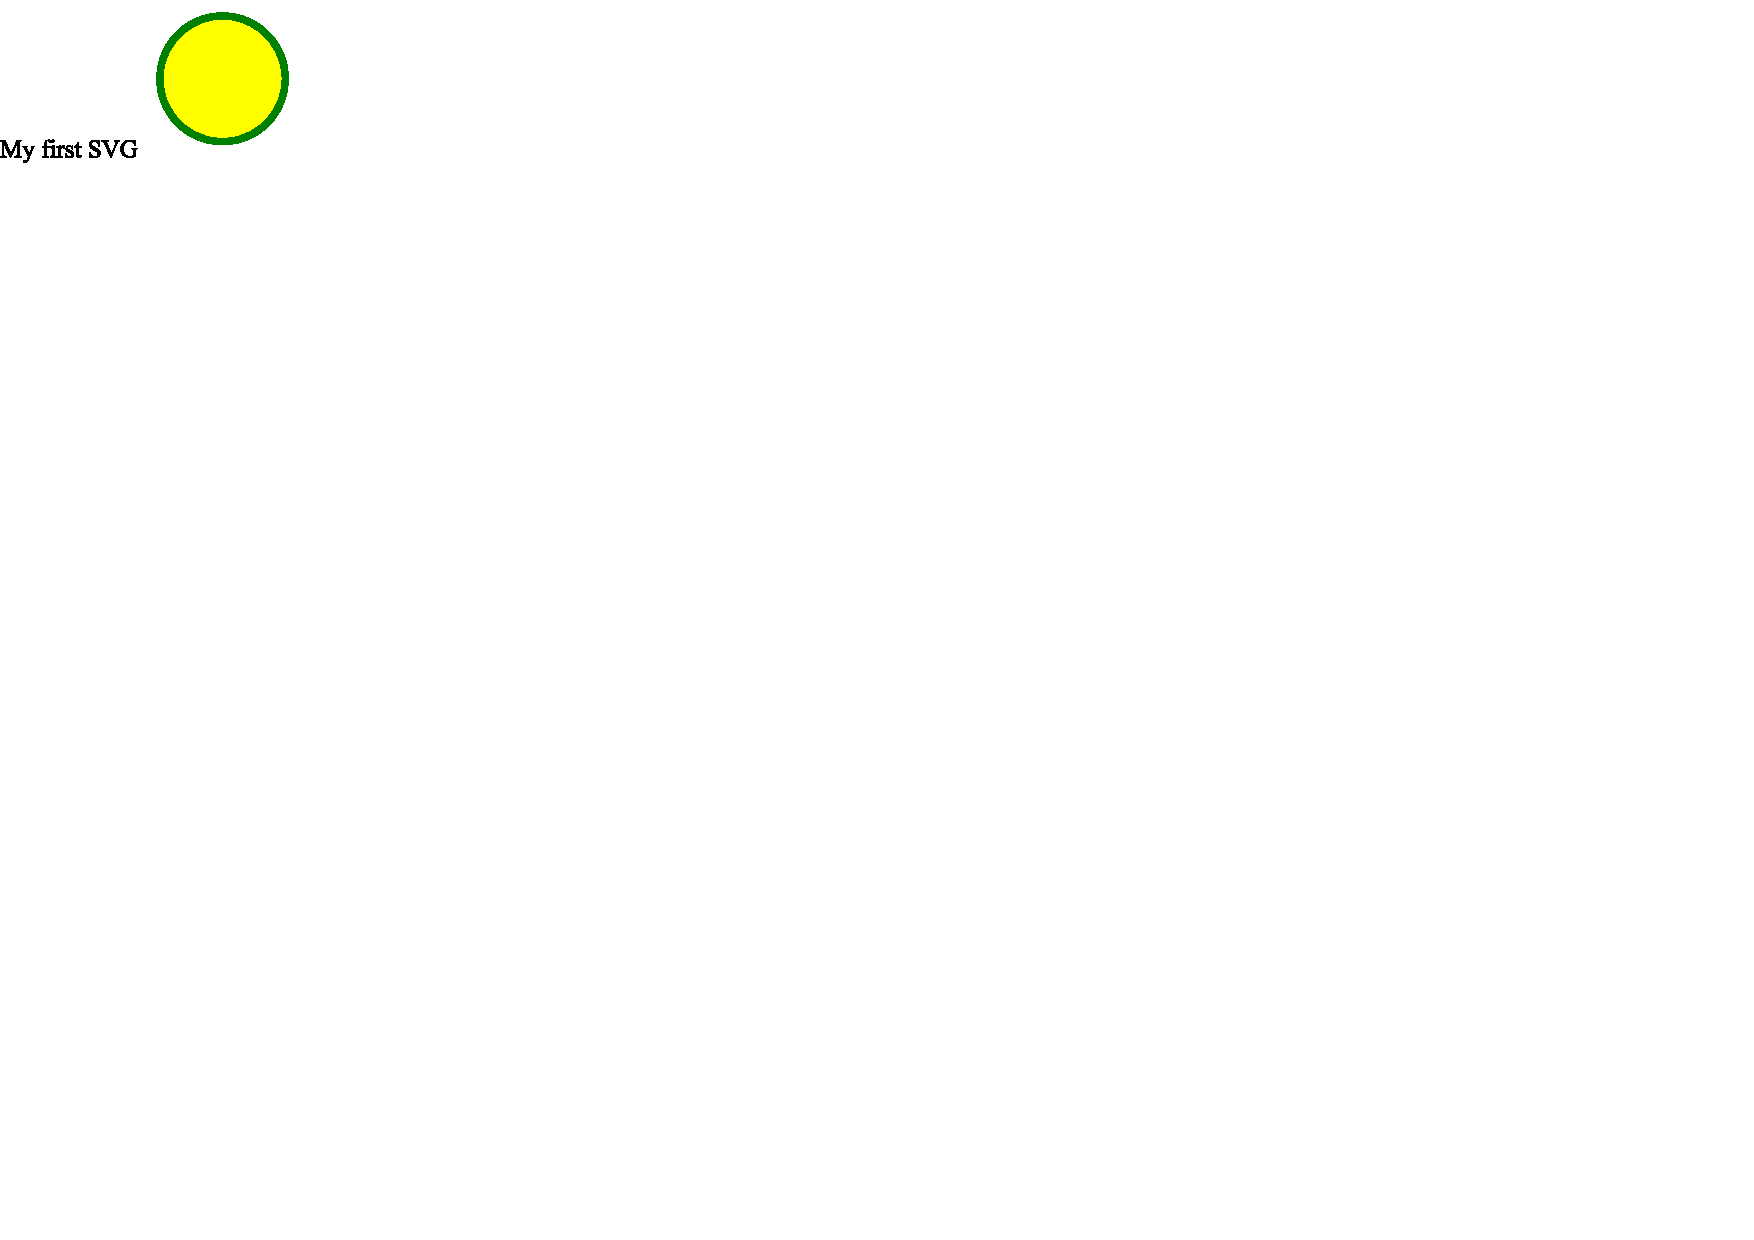
\includegraphics[width=\textwidth, angle=0]{Kreis2.pdf}
		\end{figure}
		\newpage
	
	\subsection{Requirement2}
		\begin{figure}[h!]
		    \centering
		    \captionsetup{labelformat=empty}
		    \caption{Your caption}
		    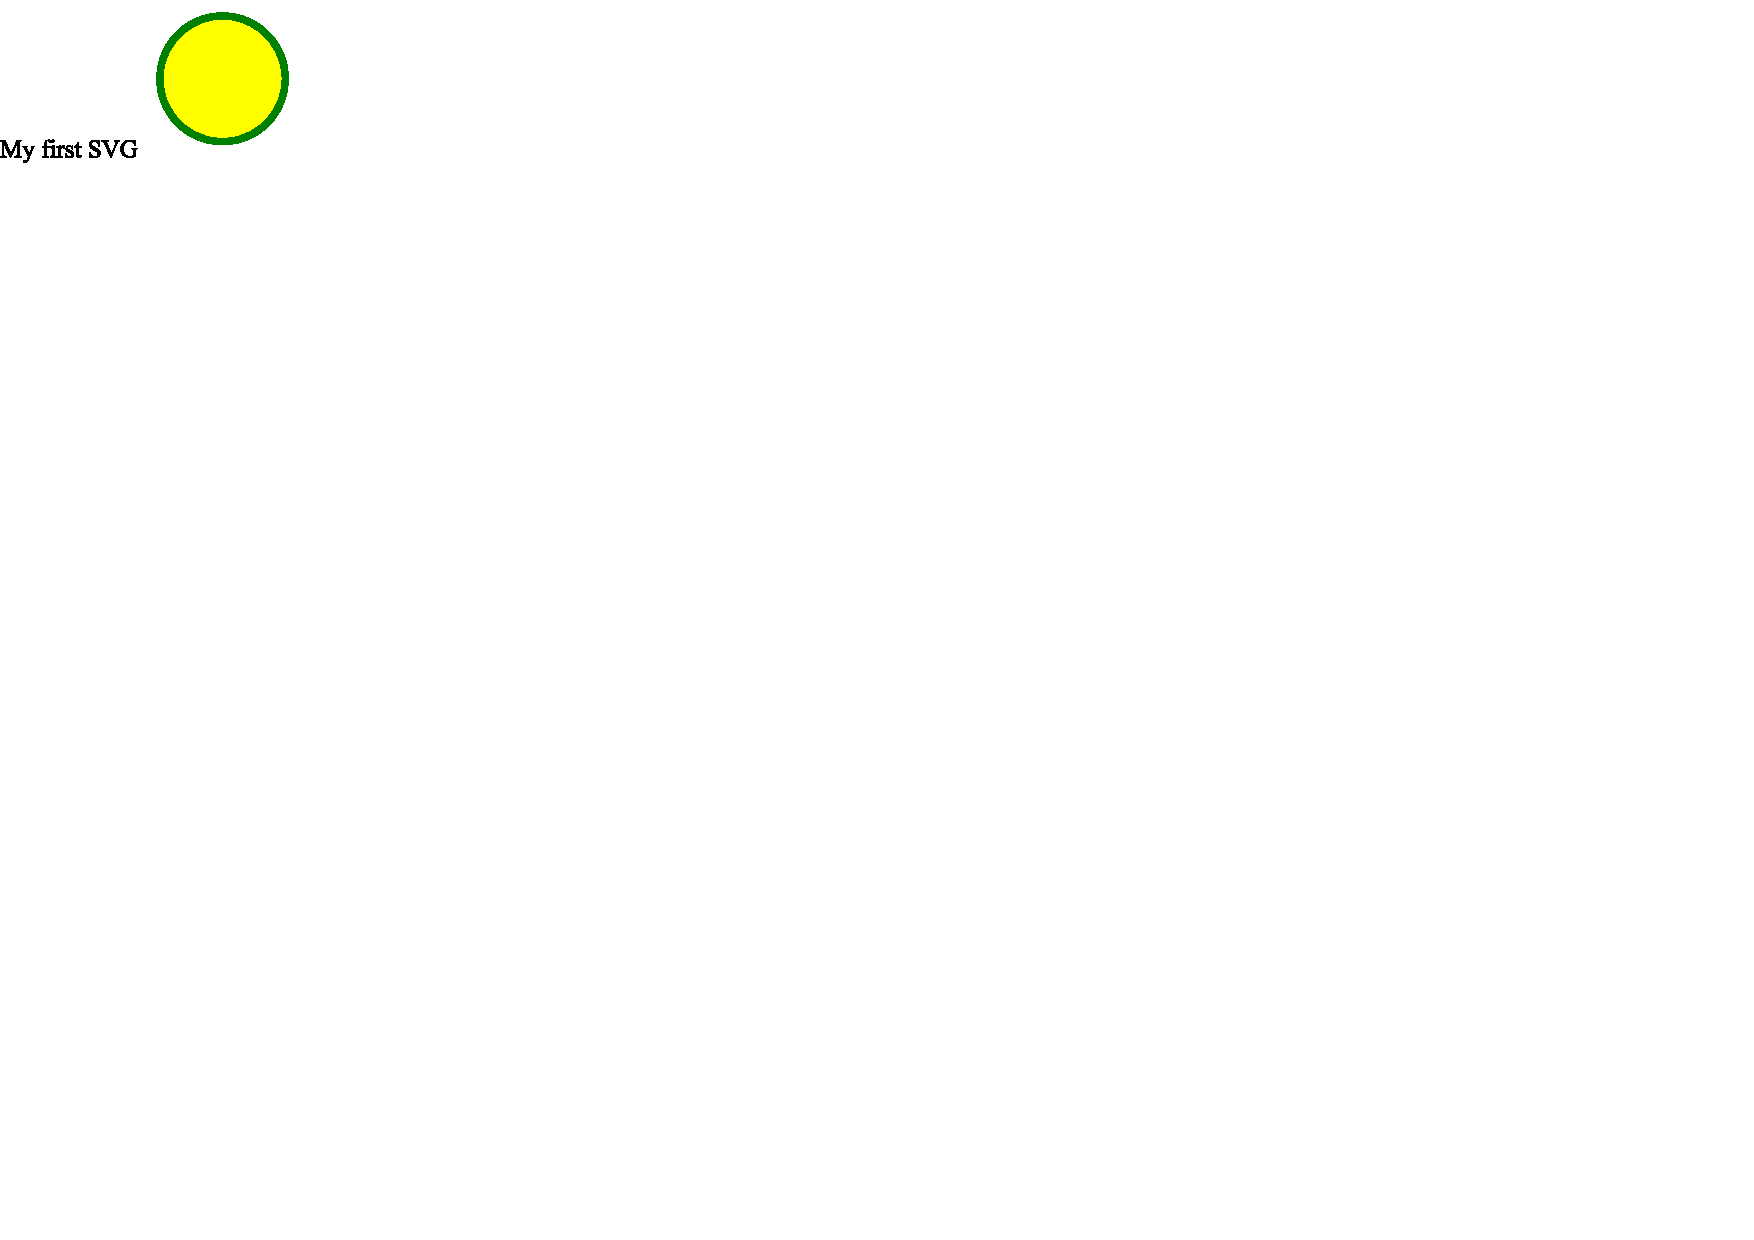
\includegraphics[width=\textwidth, angle=0]{Kreis2.pdf}
		\end{figure}
		\newpage

\section{Howard-Yi Hong Soon}

	\subsection{Requirement1}
		\begin{figure}[h!]
		    \centering
		    \captionsetup{labelformat=empty}
		    \caption{Your caption}
		    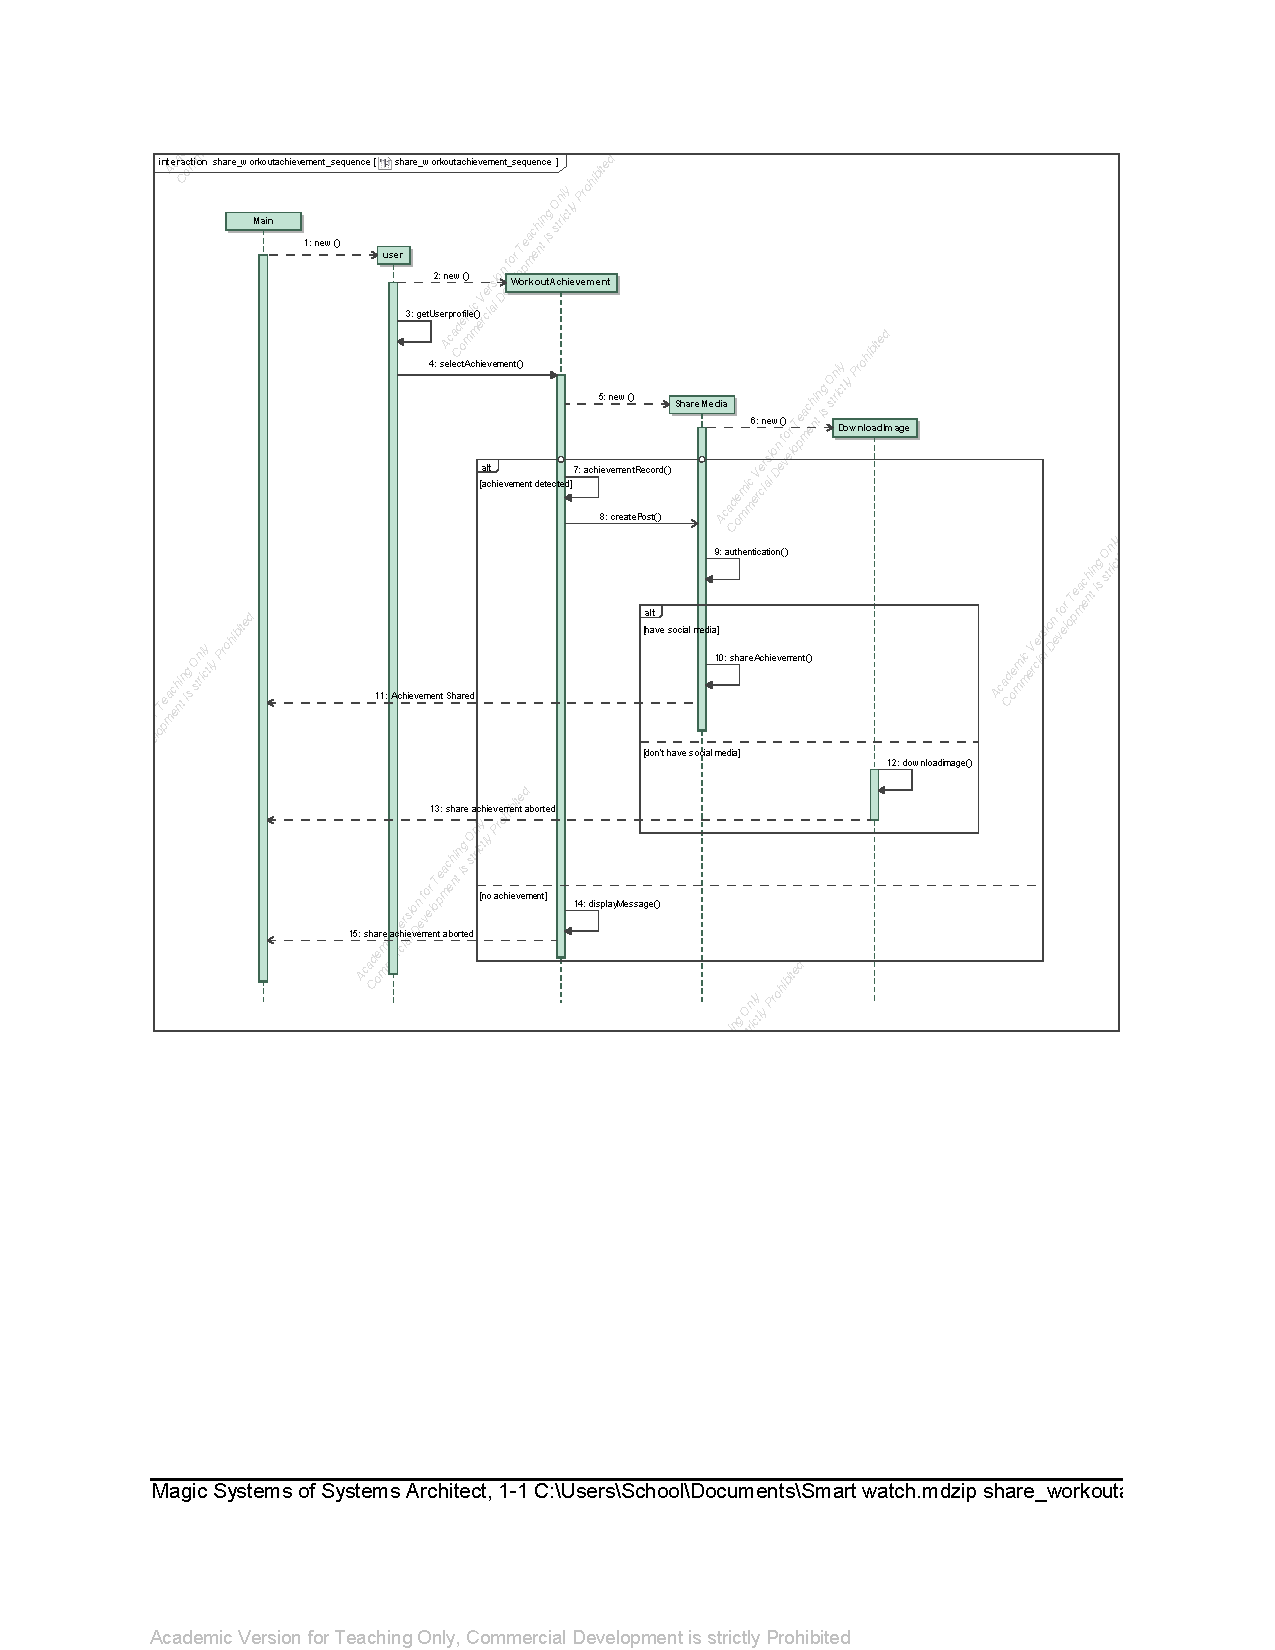
\includegraphics[width=\textwidth, angle=0]{Howard/share_workout/share_workout_sequence.pdf}
		\end{figure}
		\newpage
		\begin{figure}[h!]
		    \centering
		    \captionsetup{labelformat=empty}
		    \caption{Your caption}
		    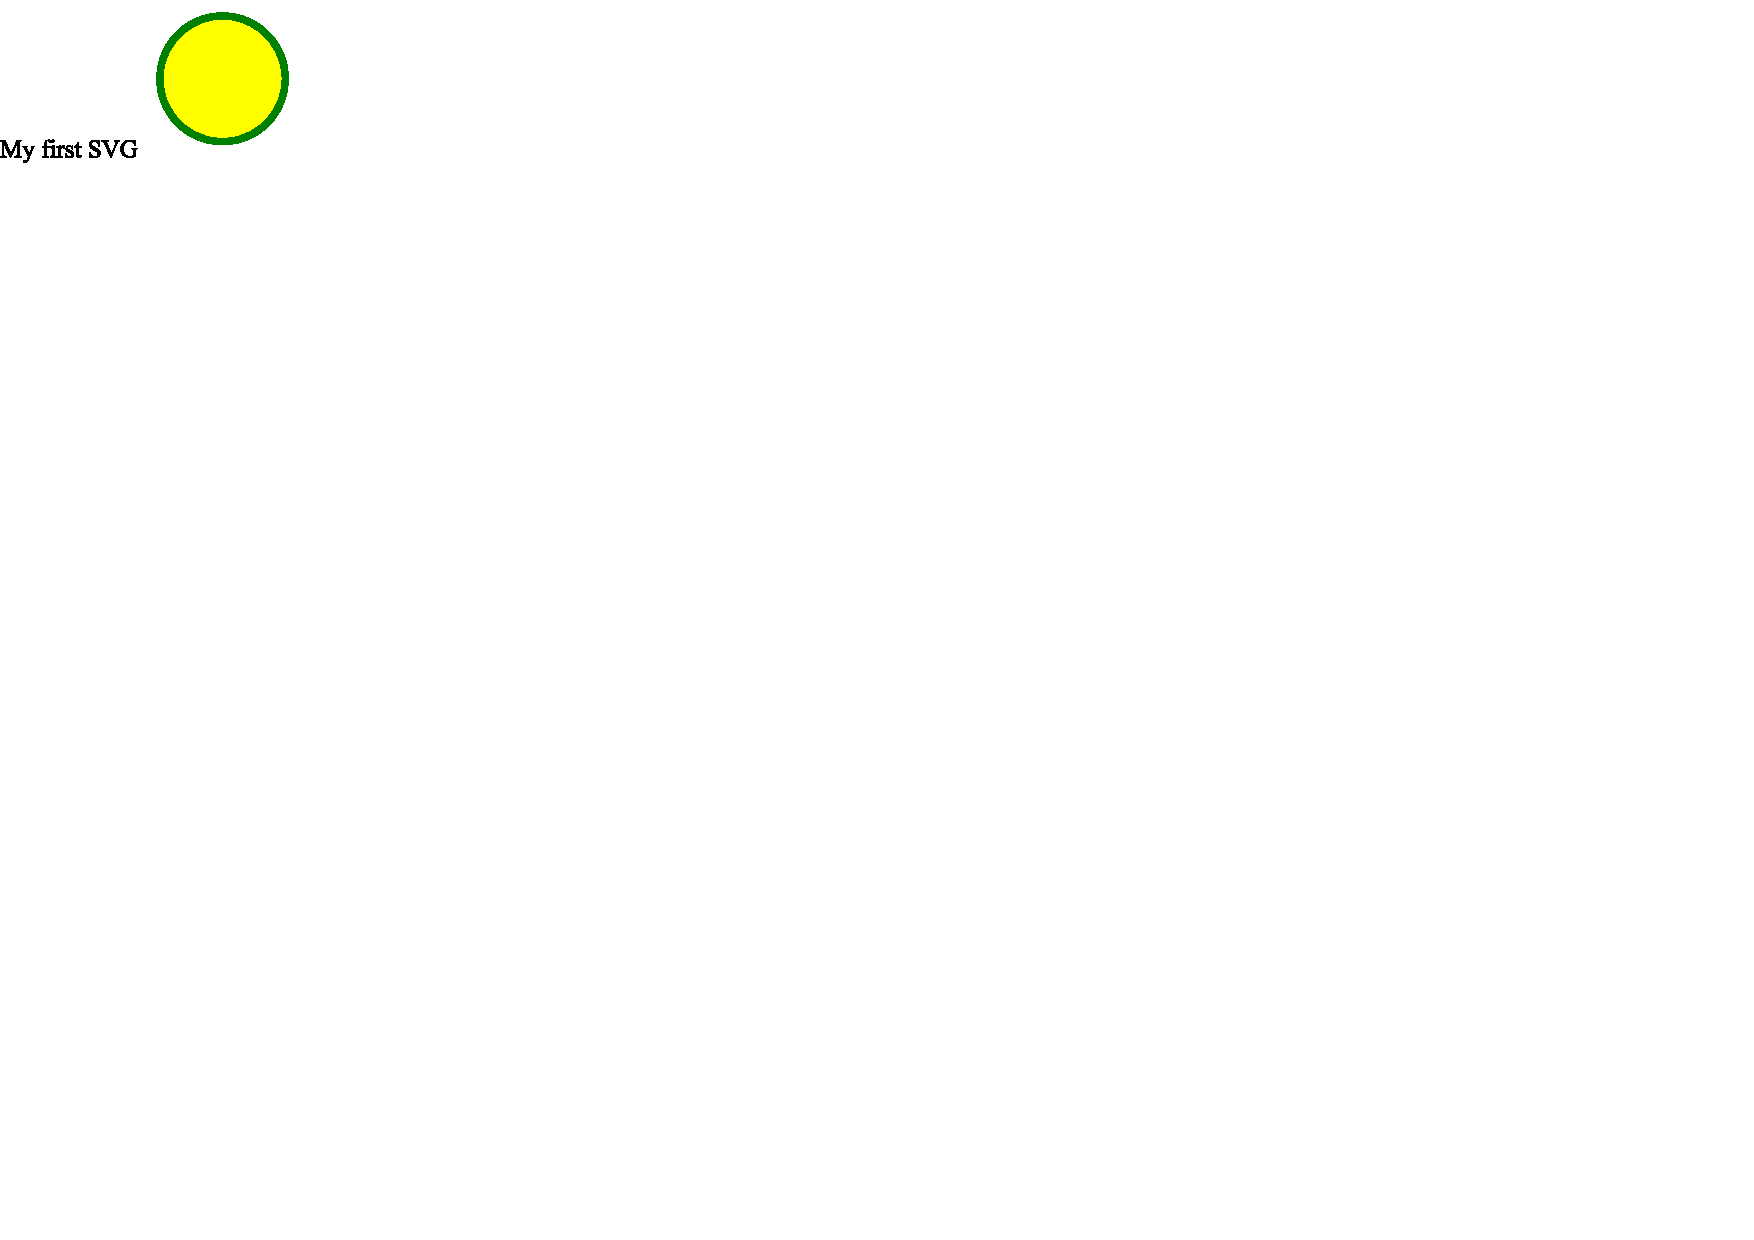
\includegraphics[width=\textwidth, angle=0]{Kreis2.pdf}
		\end{figure}
		\newpage

\section{Jiwon Won}
	\subsection{Requirement1}
		\begin{figure}[h!]
		    \centering
		    \captionsetup{labelformat=empty}
		    \caption{Your caption}
		    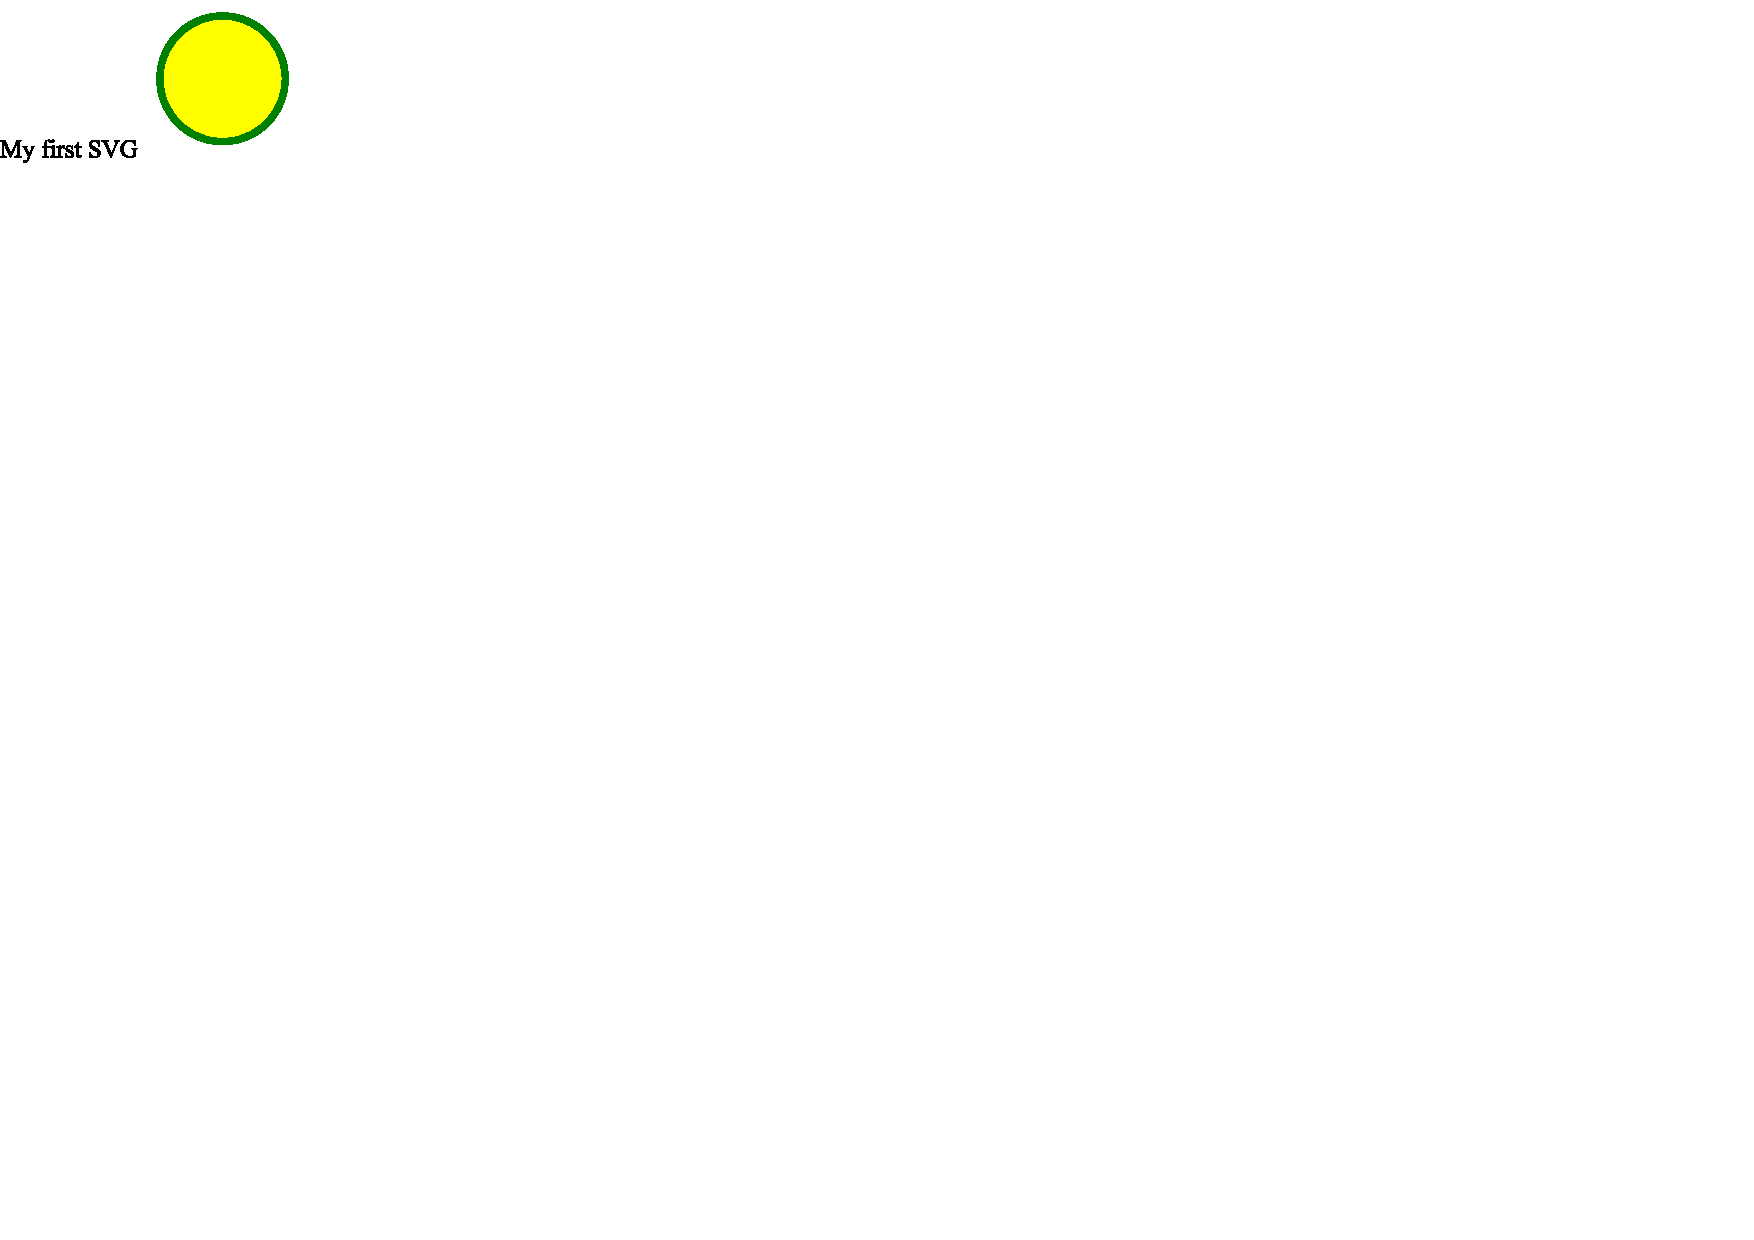
\includegraphics[width=\textwidth, angle=0]{Kreis2.pdf}
		\end{figure}
		\newpage
		\begin{figure}[h!]
		    \centering
		    \captionsetup{labelformat=empty}
		    \caption{Your caption}
		    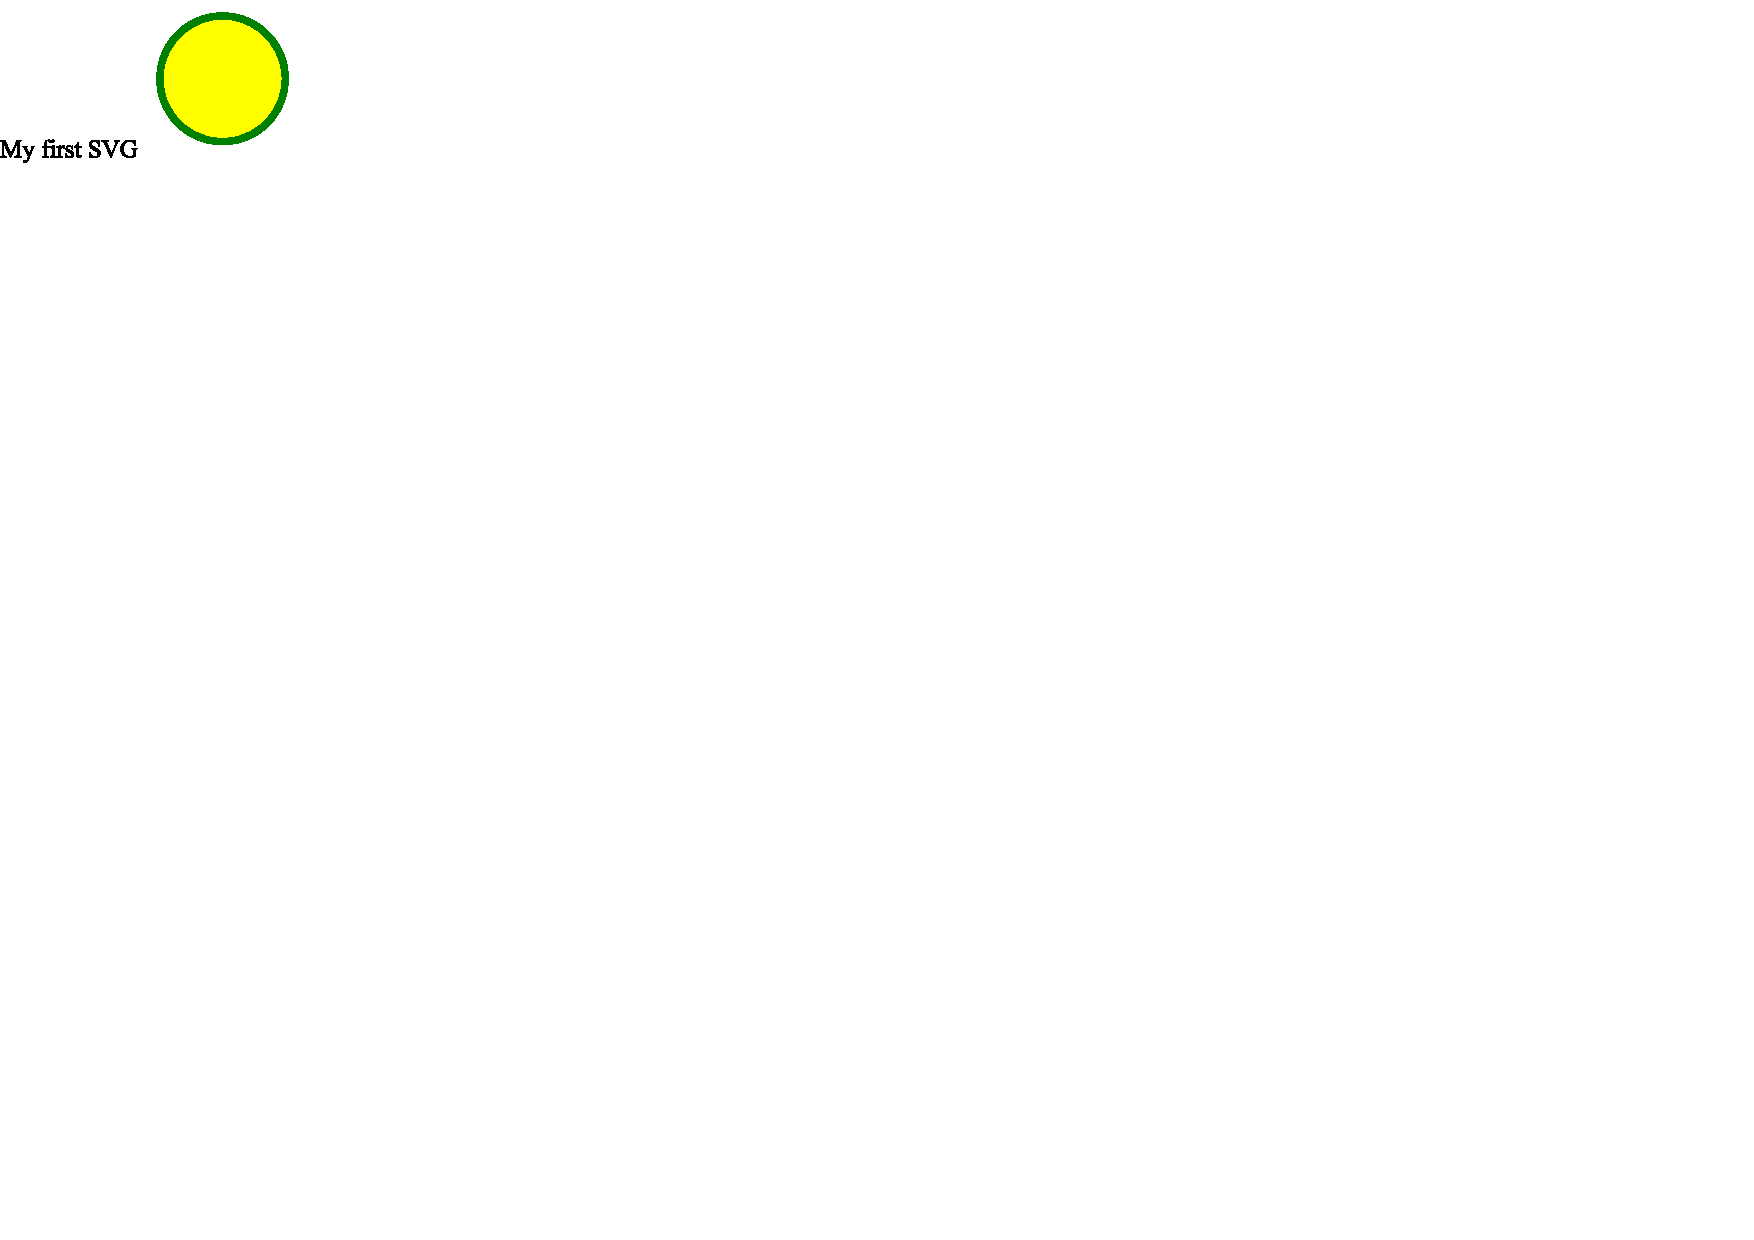
\includegraphics[width=\textwidth, angle=0]{Kreis2.pdf}
		\end{figure}
		\newpage

\section[]{Lars Friese}
	\subsection{Requirement 10: Easy usability with Gesture Control}
	\begin{center}
		\begin{tabularx}{1.0\textwidth}{|>{\raggedright\arraybackslash}p{0.2\textwidth}|>{\raggedright\arraybackslash}X|}
			\hline
			Name             & Use gestures to execute actions on smartwatch \\ \hline
			ID               & 12 \\ \hline
			Business Value   & medium \\ \hline
			Description      & When the user lifts his arm and turns his wrist the smartwatch display turns on, when he lowers the arm the display turns of. Additionally the smartwatch executes a costum gesture \\ \hline
			Trigger          & User lifting/lowering arm and turning wrist or shaking his wrist \\ \hline
			Actors           & User, System, Gyroscope Sensor\\ \hline
			Pre-conditions   & Display is turned on/off\\ \hline
			Post-conditions  & Display is turned on/off, App opened\\ \hline
			Basic Flow       & \\ \hline
							  Description & This is the main scenario where the system recognizes the hand up movement \\ \hline
							  Actions & \\ \hline
							  1 & User raises arm \\ \hline
							  2 & System recognizes gesture \\ \hline
							  3 & Display turns on \\ \hline
			Alternative Flow & A \\ \hline
							  Description & Actions \\ \hline
							  & 1 \\ \hline
							  & 2 \\ \hline
			Alternative Flow & B \\ \hline
							  Description & Actions \\ \hline
							  & 1 \\ \hline
							  & 2 \\ \hline
							  & 3 \\ \hline
							  & 4 \\ \hline
							  & 5 \\ \hline
		\end{tabularx}
	\end{center}

	\begin{figure}[htbp]
		\centering
		\begin{subfigure}{\textwidth}
			\resizebox{\textwidth}{!}{\includesvg[]{Lars/Use Case Gesture Control/GestureControl_usecase.svg}}
			\caption{Use Case Diagram}
		\end{subfigure}
		\begin{subfigure}{\textwidth}
			Example text 1 \\
			Example text 2
		\end{subfigure}
	\end{figure}
	
	\begin{figure}[htbp]
		\centering
		\begin{subfigure}{\textwidth}
			\resizebox{\textwidth}{!}{\includesvg[]{Lars/Use Case Gesture Control/GestureControl_activity.svg}}
			\caption{Activity Diagram}
		\end{subfigure}
		\begin{subfigure}{\textwidth}
			Example text 3 \\
			Example text 4
		\end{subfigure}
	\end{figure}
	
	\begin{figure}[htbp]
		\centering
		\begin{subfigure}{\textwidth}
			\resizebox{\textwidth}{!}{\includesvg[]{Lars/Use Case Gesture Control/GestureControl_class.svg}}
			\caption{Class Diagram}
		\end{subfigure}
		\begin{subfigure}{\textwidth}
			Example text 5 \\
			Example text 6
		\end{subfigure}
	\end{figure}
	
	\begin{figure}[htbp]
		\centering
		\begin{subfigure}{\textwidth}
			\resizebox{\textwidth}{!}{\includesvg[]{Lars/Use Case Gesture Control/GestureControl_sequence.svg}}
			\caption{Sequence Diagram}
		\end{subfigure}
		\begin{subfigure}{\textwidth}
			Example text 7 \\
			Example text 8
		\end{subfigure}
	\end{figure}
\newpage


\section{Marc Roemer}
	\subsection{Requirement 9: Calculation and display daily and weekly step count statistics}
		\begin{figure}[h!]
			\centering
			\captionsetup{labelformat=empty}
			\caption{UseCase}
		\end{figure}
		\newpage
		\begin{figure}[h!]
			\centering
			\captionsetup{labelformat=empty}
			\caption{UI Prototype}
		\end{figure}
		\newpage
		\begin{figure}[h!]
		    \centering
		    \captionsetup{labelformat=empty}
		    \caption{Activity Diagram}
		    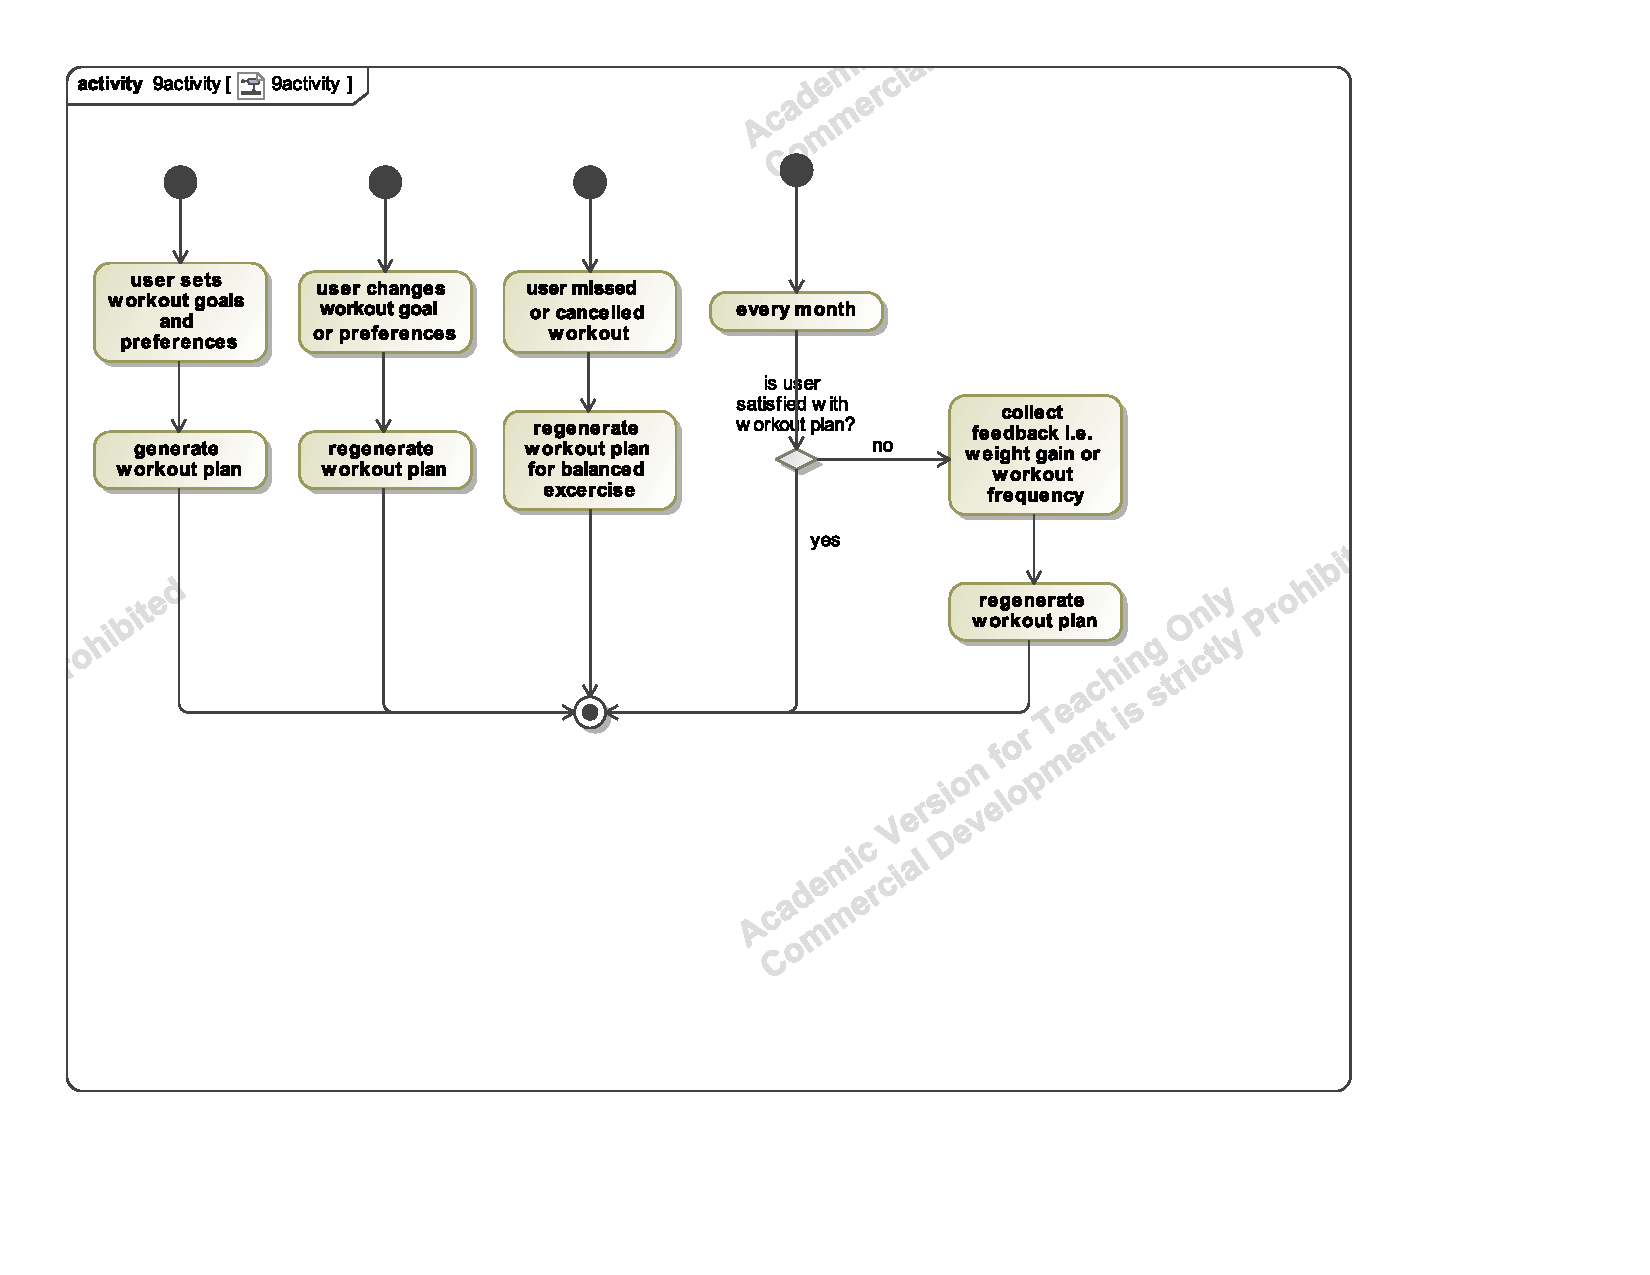
\includegraphics[width=\textwidth, angle=0]{Marc/req9/9activity.pdf}
		\end{figure}
		\newpage
		\begin{figure}[h!]
			\centering
			\captionsetup{labelformat=empty}
			\caption{UseCase Diagram}
		\end{figure}
		\newpage
		\begin{figure}[h!]
			\centering
			\captionsetup{labelformat=empty}
			\caption{Sequence Diagram}
		\end{figure}
		\newpage
		\begin{figure}[h!]
			\centering
			\captionsetup{labelformat=empty}
			\caption{Class Diagram}
		\end{figure}
		\newpage

	\subsection{Requirement 10: Create and manages a workout plan}
		\begin{figure}[h!]
			\centering
			\captionsetup{labelformat=empty}
			\caption{UseCase}
		\end{figure}
		\newpage
		\begin{figure}[h!]
			\centering
			\captionsetup{labelformat=empty}
			\caption{UI Prototype}
		\end{figure}
		\newpage
		\begin{figure}[h!]
		    \centering
		    \captionsetup{labelformat=empty}
		    \caption{Activity Diagram}
		    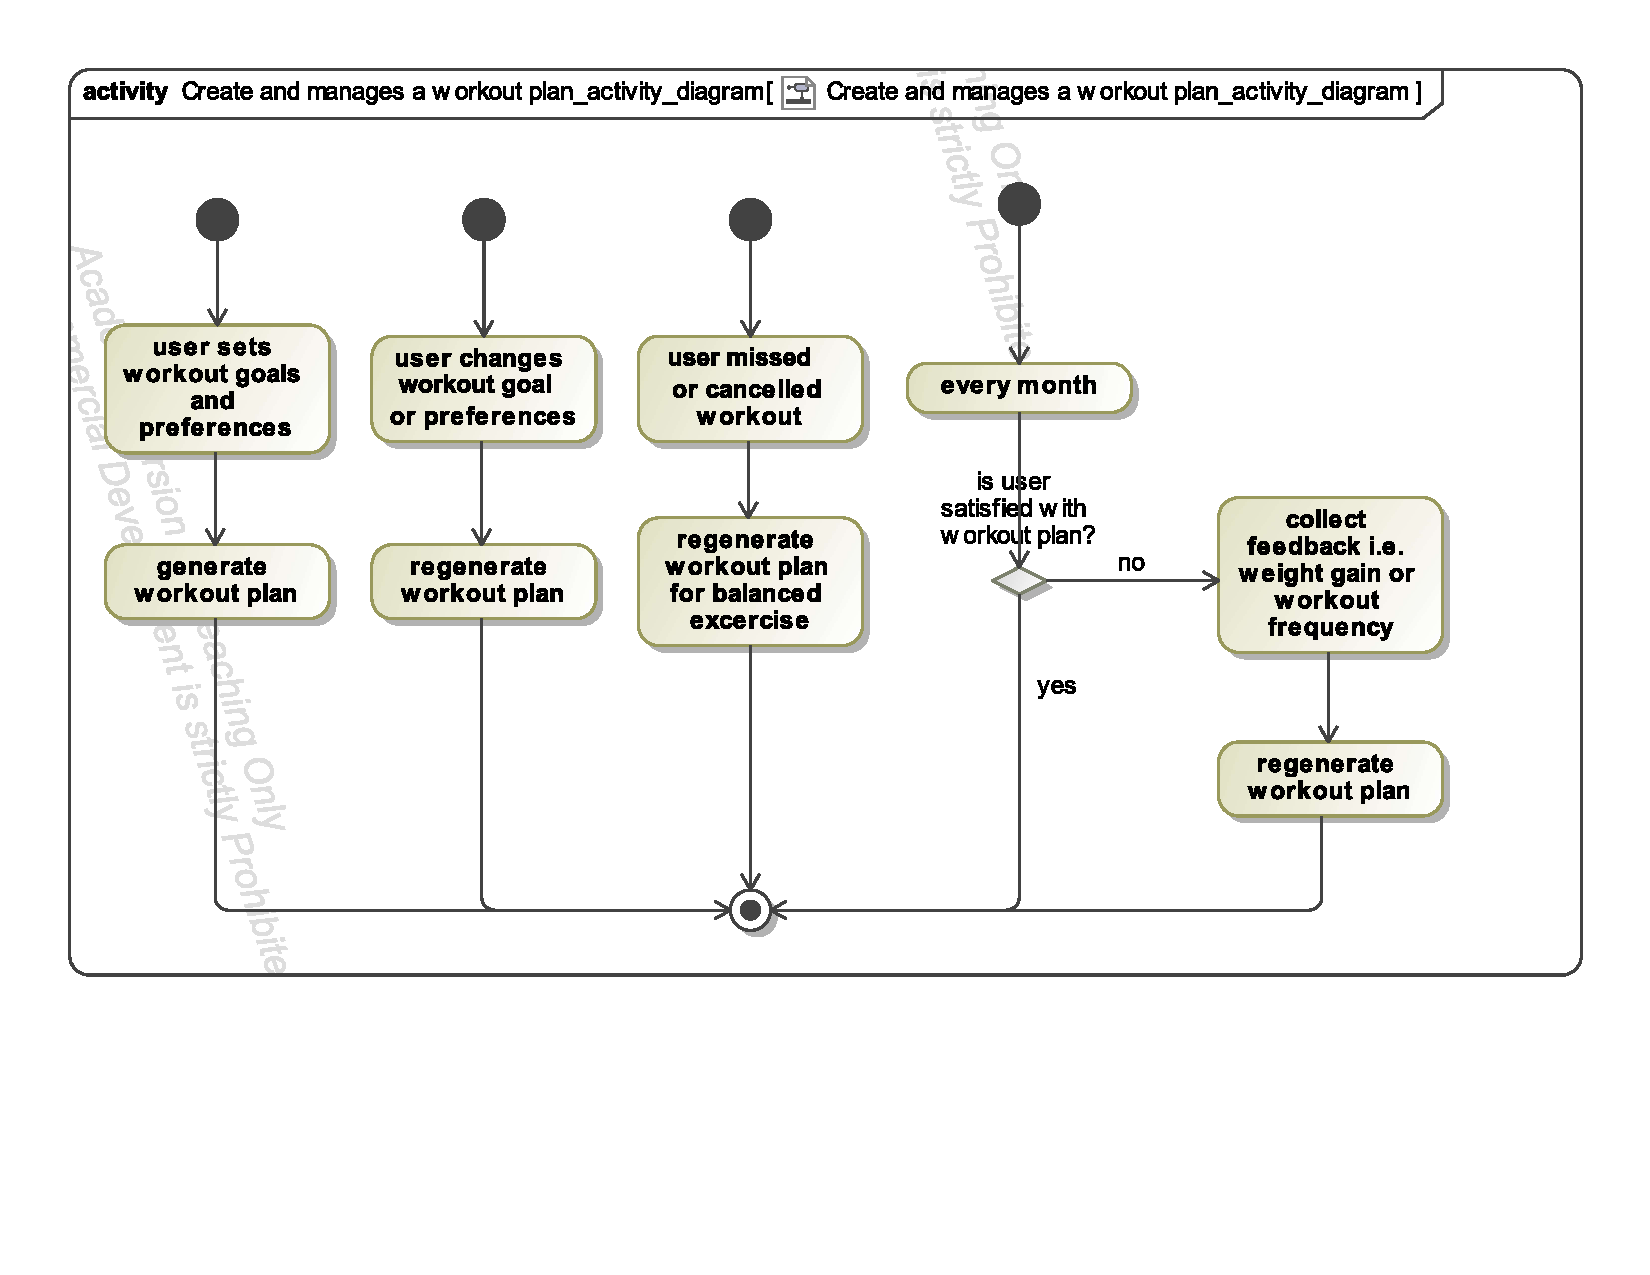
\includegraphics[width=\textwidth, angle=0]{Marc/req10/10activity.pdf}
		\end{figure}
		\newpage
		\begin{figure}[h!]
			\centering
			\captionsetup{labelformat=empty}
			\caption{UseCase Diagram}
		\end{figure}
		\newpage
		\begin{figure}[h!]
			\centering
			\captionsetup{labelformat=empty}
			\caption{Sequence Diagram}
		\end{figure}
		\newpage
		\begin{figure}[h!]
			\centering
			\captionsetup{labelformat=empty}
			\caption{Class Diagram}
		\end{figure}
		\newpage
			

\section{Stefan Nguyen}
	\subsection{Requirement 11: Environment Monitoring }
		
		\begin{center}
			\begin{tabularx}{1.0\textwidth}{|>{\raggedright\arraybackslash}p{0.2\textwidth}|>{\raggedright\arraybackslash}X|}
				\hline
				Name             & Environment monitoring \\ \hline
				ID               & 11 \\ \hline
				Business Value   & Low \\ \hline
				Description      & Tracks UV exposure, air quality, temperature in real time \\ \hline
				Trigger          & Typical event which adjusts the changes in real time \\ \hline
				Actors           & Environmental Sensor Array, which is responsible for capturing environmental data \\ \hline
				Pre-conditions   & Environmental sensors are operational and calibrated\\ \hline
				Post-conditions  & Displays the data in the smartwatch\\ \hline
				Basic Flow       & \\ \hline
								  Description & Detail each change in the environment monioring system \\ \hline
								  Actions & \\ \hline
								  1 & activating the sensors \\ \hline
								  2 & capturing the data (e.g. temperature, UV, etc) \\ \hline
								  3 & processing data e.g. analysis or computations \\ \hline
								  4 & transfer data into smartwatch \\ \hline
								  5 & display data in smartwatch \\ \hline
				Alternative Flow & A \\ \hline
								  Description & Error capturing data (network, communication etc) \\ \hline
								  1 & sensor fails to capture data \\ \hline
								  2 & fail, communication or network error in smartwatch or sensor \\ \hline
								  3 & Error capturing data / false data display information \\ \hline
				Alternative Flow & B \\ \hline
								  Description & Environmental sensor detect conditions which my threaten health conditions \\ \hline
								  1 & sensor detects hazardous condition and flag it as highest priority \\ \hline
								  2 & sends push notification and warns the user \\ \hline
								  3 & displays the notification on the smartwatch and recommends actions (e.g. apply sunscreen, seek shelter, etc) \\ \hline
								  4 & user acknowledges the notification\\ \hline
								  5 & user doesn't acknoweldege notification -> the system keeps sending notifications or warns the user \\ \hline
			\end{tabularx}
		\end{center}
		\newpage
\end{document}